%卒論概要テンプレート ver. 4.0

\documentclass[uplatex,twocolumn,dvipdfmx]{jsarticle}
\usepackage[top=22mm,bottom=22mm,left=22mm,right=22mm]{geometry}
\setlength{\columnsep}{11mm}
\usepackage[T1]{fontenc}
\usepackage{txfonts}
\usepackage[expert,deluxe]{otf}
\usepackage[dvipdfmx,hiresbb]{graphicx}
\usepackage[dvipdfmx]{hyperref}
\usepackage{pxjahyper}
\usepackage{secdot}





%タイトルと学生番号,名前だけ編集すること
\title{\vspace{-5mm}\fontsize{14pt}{0pt}\selectfont TwitterのRTシュミレーション}
\author{\normalsize プロジェクトマネジメントコース 矢吹研究室 1442043 川崎貴雅}
\date{}
\pagestyle{empty}

\begin{document}
\fontsize{10.5pt}{\baselineskip}\selectfont
\maketitle





%以下が本文
\section{序論}\label{序論}

スマートフォンなどの普及と共にTwitterやFecebookを始めとしたとしたマイクロブログが急激に普及している.特にTwitterはリアルタイムな情報を手軽に多くのユーザーへと伝播できるため社会に影響を与えている.例えば東日本大震災時のデマ情報が拡散された事や北朝鮮のミサイルを目撃したというデマが挙げられる\cite{ミサイルのデマ画像がTwitterで拡散「北朝鮮のミサイルが見えた」}.このような拡散されたツイートをシュミレーションで再現することができるのではないかと考えられる.

本研究では現実のTwitterを調査し,現実に近いRTのシュミレーションで再現することができるかを調査したい.
今回は3段階に分けて行う.1つ目は1日のツイート数の分布を出す.2つ目にランダムグラフを用いたRTのシュミレーションを行う.最後に1つ目と2つ目を合わせて現実の条件に近づける.


\section{目的}

本研究ではRTのシュミレーションを1日のツイート数の分布やランダムグラフを用いたRTのシュミレーションを行い,現実に近い状況をシュミレーションで再現を行えるかを調査する.

\section{手法}

RTのシュミレーションを現実に近いシュミレーションするうえで以下の手法で行う.

\begin{enumerate}
\item TwitterAPIを用いてツイートを取得し,CSVファイルを作成する.
\item CSVファイルをGitHubGistでURLでインポートできるようにし,WOLFRAM CLOUDで処理を行い1日あたりのツイート数の平均を求める.
\item RTのシュミレーションの流れをつかむためにグループ作成にランダムグラフを用いたシュミレーションを行う.
\item 現実に近いシュミレーションにするため改良を行う.
\end{enumerate}


\section{結果}

作成されたCSVファイルから1日あたりのツイート数の平均は1.37542回であることが分かった,またランダムグラフを用いたシュミレーションを行うことができた.


\begin{figure}[htb]
\centering
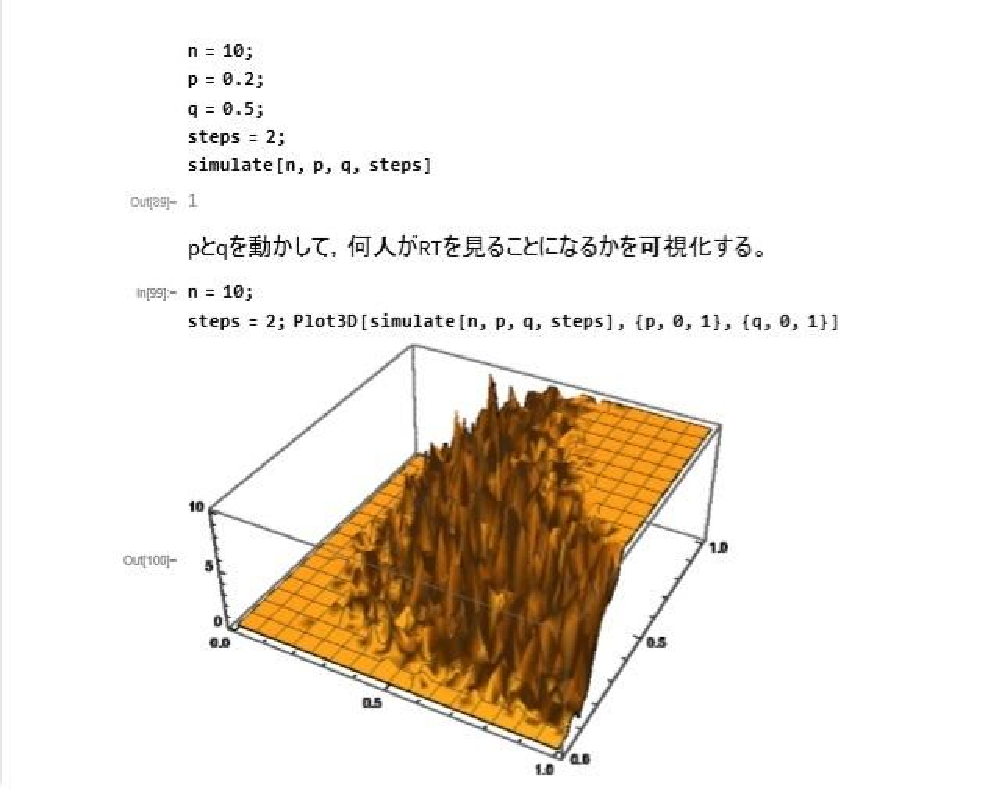
\includegraphics[width=66mm,clip]{rtsyumi.pdf}
\caption{シュミレーション結果を可視化したもの}\label{サンプル図}
\end{figure}

\section{考察}

現実に近いシュミレーションを行う上で,Twitterのユーザー間のフォロワーを判別しグループの作成ができれば,1日の平均ツイート数と合わせてシュミレーションをすることができたのではないのかと考えられる.

\section{結論}

本研究では1日あたりのツイート数の平均が分かったこととランダムグラフによるグループ内でのRTシュミレーションを行うことができた.現実に近いシュミレーションを行うにはTwitterのユーザー間のフォロワーの情報や平均RT数がわかればより現実に近いシュミレーションができることが期待される.

\bibliographystyle{junsrt}
\bibliography{biblio}%「biblio.bib」というファイルが必要.

\end{document}
